\documentclass[english,11pt]{beamer}

\DeclareMathOperator{\Cov}{Cov}
\DeclareMathOperator{\Var}{Var}
\DeclareMathOperator{\E}{\mathbb{E}}
\DeclareMathOperator{\Proba}{\mathbb{P}}

\newcommand{\Covb}[2]{\ensuremath{\Cov\!\left[#1,#2\right]}}
\newcommand{\Eb}[1]{\ensuremath{\E\!\left[#1\right]}}
\newcommand{\Pb}[1]{\ensuremath{\Proba\!\left[#1\right]}}
\newcommand{\Varb}[1]{\ensuremath{\Var\!\left[#1\right]}}

% norm
\newcommand{\norm}[1]{\| #1 \|}

\newcommand{\indep}{\rotatebox[origin=c]{90}{$\models$}}





\usepackage{mathptmx,amsmath,amssymb,graphicx,bibentry,bbm,babel,ragged2e}

\makeatletter

\newcommand{\noun}[1]{\textsc{#1}}
\newcommand{\jitem}[1]{\item \begin{justify} #1 \end{justify} \vfill{}}
\newcommand{\sframe}[2]{\frame{\frametitle{#1} #2}}

\newenvironment{centercolumns}{\begin{columns}[c]}{\end{columns}}
%\newenvironment{jitem}{\begin{justify}\begin{itemize}}{\end{itemize}\end{justify}}

\usetheme{Warsaw}
\setbeamertemplate{footline}[text line]{}
\setbeamercolor{structure}{fg=purple!50!blue, bg=purple!50!blue}

\setbeamersize{text margin left=15pt,text margin right=15pt}

\setbeamercovered{transparent}


\@ifundefined{showcaptionsetup}{}{%
 \PassOptionsToPackage{caption=false}{subfig}}
\usepackage{subfig}

\usepackage[utf8]{inputenc}
\usepackage[T1]{fontenc}

\usepackage{multirow}


\makeatother

\begin{document}





\title{Innovation dynamics in multi-scalar systems of cities}

\author{J.~Raimbault$^{1,2,3,4,\ast}$ and D. Pumain$^4$\\
\texttt{$\ast$ juste.raimbault@ign.fr}
}


\institute{$^{1}$ LASTIG, IGN-ENSG\\
$^{2}$CASA, UCL\\
$^{3}$UPS CNRS 3611 ISC-PIF\\
$^{4}$UMR CNRS 8504 G{\'e}ographie-cit{\'e}s
}


\date{ALife 2023 - ALife and Society\\\smallskip
July 28th 2023
}

\frame{\maketitle}




\sframe{Urban dynamics and innovation}{

\justify

	$\rightarrow$ Cities are central for innovation in social systems \cite{pumain2020theories} and future sustainability \cite{keith2022newshort}
	
	\bigskip
	
	$\rightarrow$ Urban innovation systems now span from local clusters to global networks \cite{binz2017global}
	
	\bigskip
	
	$\rightarrow$ Innovation dynamics in systems of cities follow complex patterns across scales \cite{bauer2019local}
	


}


\sframe{Towards multi-scalar models}{


\justify

	$\rightarrow$ Multi-scalar models necessary to design sustainable territorial policies \cite{rozenblat2018conclusion}
          
         \bigskip      
                
	$\rightarrow$ ``Artificial cities'' \cite{raimbault2020cities} and urban simulation approaches focus on a single scale
	
	  \bigskip 
	   \bigskip 

\textbf{Contribution: } a new \textbf{simulation model} coupling innovation diffusion dynamics \textbf{between cities} (macro) \cite{raimbault2020modelshort} with research cluster dynamics \textbf{within urban areas} (meso) \cite{raimbault2022innovationshort}


}


\sframe{Macroscopic dynamics}{

\begin{center}
	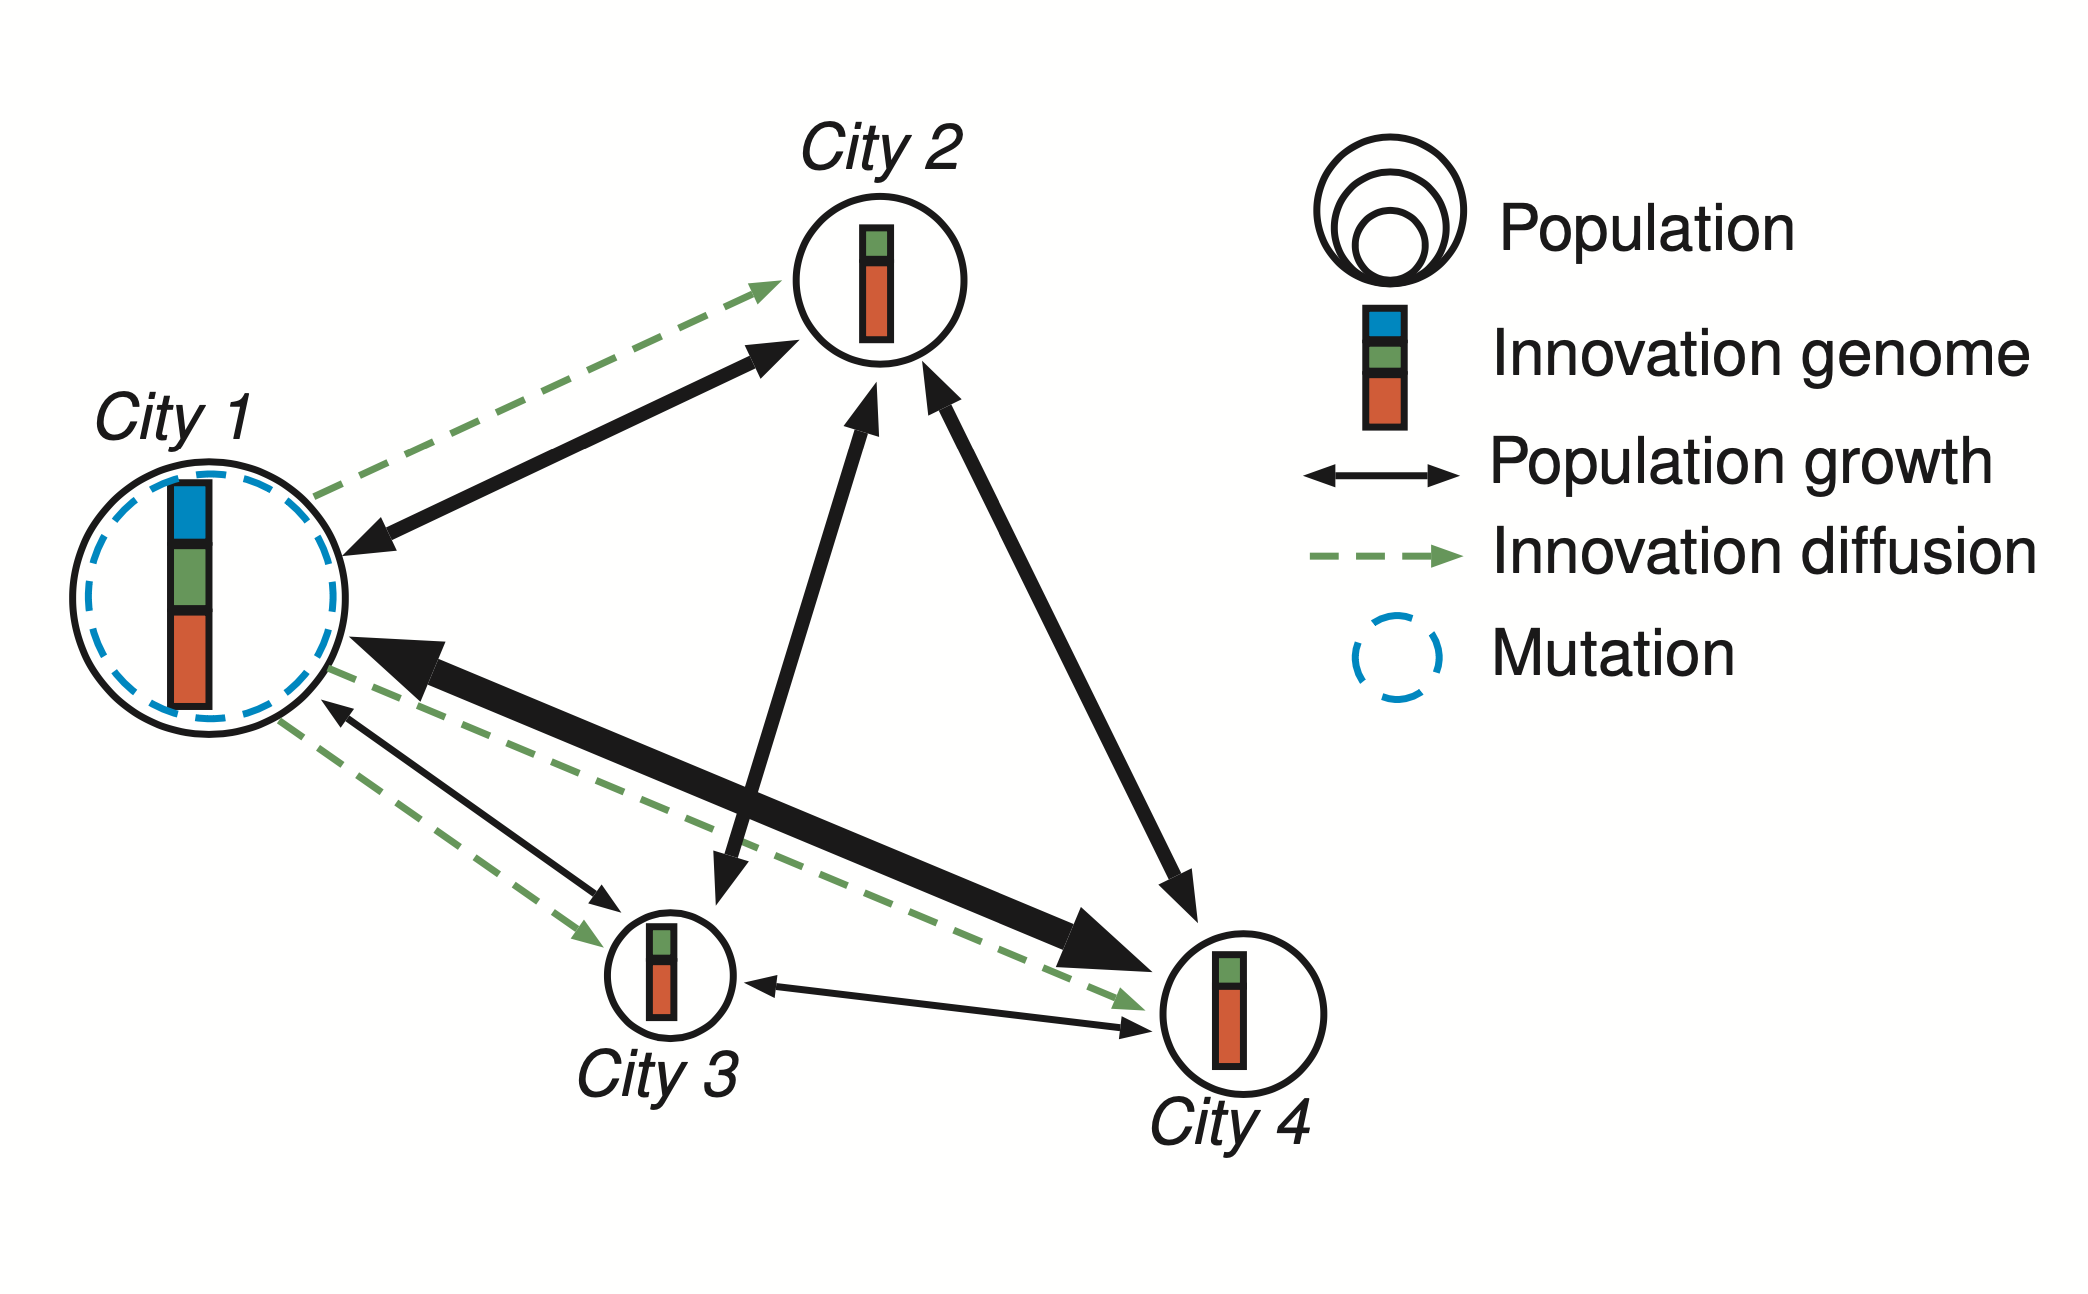
\includegraphics[width=\textwidth]{figures/model_4}	
\end{center}

\footnotesize

Raimbault, J. (2020). A model of urban evolution based on innovation diffusion. In Artificial Life Conference Proceedings 32 (pp. 500-508).

}

\sframe{Mesoscopic dynamics}{

\justify

Mesoscopic dynamics from \cite{raimbault2022innovation}: \textbf{Innovation clusters} composed of firms, sets of employees (real-valued genome representing ideas); aim at optimising a fixed random fitness (Rastrigin function).

\bigskip

\textbf{Meso cycle:} in each innovation cluster (city) for $t_m$ meso time steps:

    \begin{itemize}
        \item employee exchange ideas within firms (genome crossovers)
        \item idea with best fitness is chosen by each company
        \item ideas are informally exchanged between firms
	\end{itemize}

}

\sframe{Inter-scale dynamics}{

\justify

\textbf{Iterated steps}, for $t_f$ macro time steps:

            \begin{enumerate}
\item Mesoscopic cycle
\item \textbf{Bottom-up feedback:} if relative fitness gain of the best firm exceeds a parameter  ($\delta f_i > \theta$), the corresponding city will innovate at the macro scale.
\item Macroscopic step: innovation diffusion; population migration and growth; new innovations.
\item \textbf{Top-down feedback:} firm strategy is updated by changing crossover probability and mutation probability, and the urban environment in terms of informal exchanges, both depending on relative population growth.
\end{enumerate}


}


\sframe{Model indicators}{

\begin{itemize}
	\item Macro observables: utility and diversity of innovations
    \item Meso observables: best fitness and diversity of ideas
    \item Indicators for downward causation from \cite{rosas2020reconcilingshort} on these observables to quantify the strength of emergence: ($\Delta$, $\Psi$, $\Gamma$)
\end{itemize}

\bigskip

\textbf{Model setup} on synthetic systems of cities resembling real systems \cite{raimbault2019space}

}


\sframe{Model implementation}{

Model implemented in scala: \url{https://github.com/JusteRaimbault/InnovationMultiscale-model}

\bigskip

Integrated into the OpenMOLE platform for \textbf{model exploration and validation}	\cite{reuillon2013openmole}

\medskip

\begin{center}

\includegraphics[width=0.15\textwidth]{figures/iconOM.png}

\includegraphics[width=0.55\textwidth]{figures/openmole.png}
\end{center}


}

\sframe{Model exploration}{

\begin{center}
	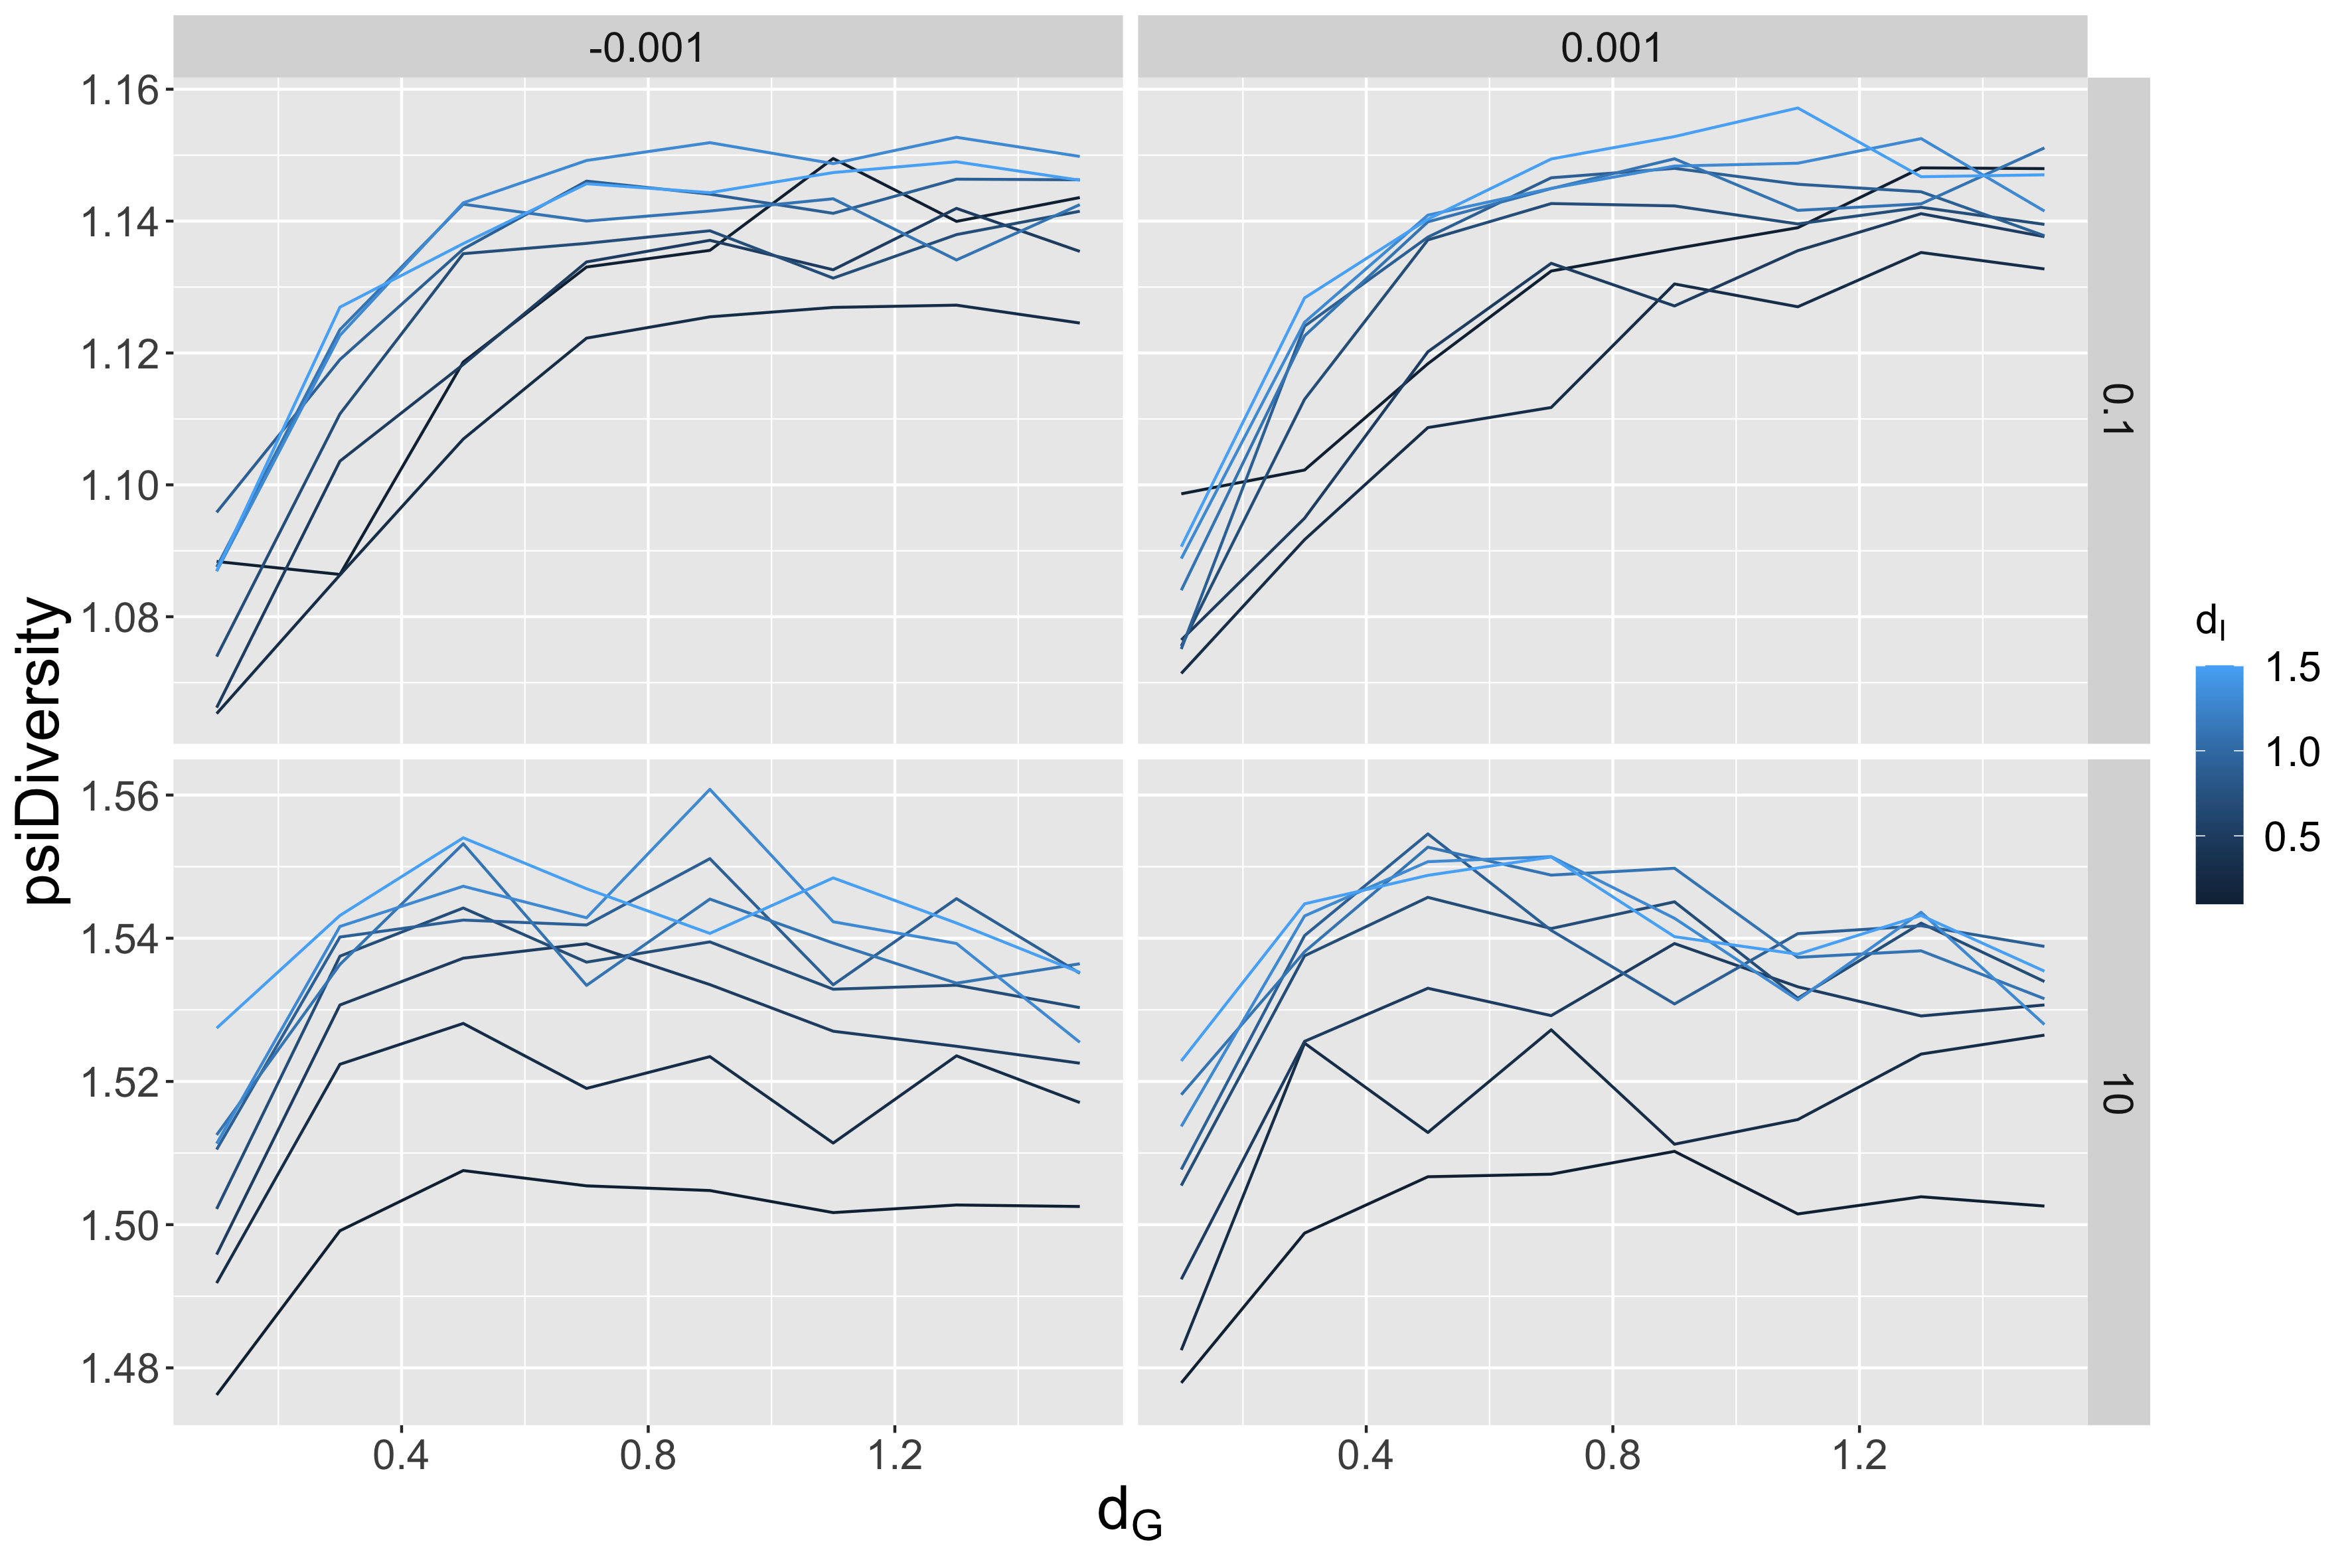
\includegraphics[width=0.87\linewidth]{../poster/figures/psiDiversity-macroGravityDecay_color-macroInnovationDecay_facet-mesoToMacroInnovationThreshold-macroToMesoExchangeMaxUpdate_mesoCrossOverProba0-5.png}	
\end{center}

\smallskip

\footnotesize

\textit{Increasing then plateauing strength of emergence $\Psi$ for macro diversity, as a function of spatial interaction range $d_G$ and innovation diffusion range $d_I$, for varying top-down (columns) and bottom-up (rows) feedbacks.}

}

\sframe{Model optimisation}{

\begin{center}
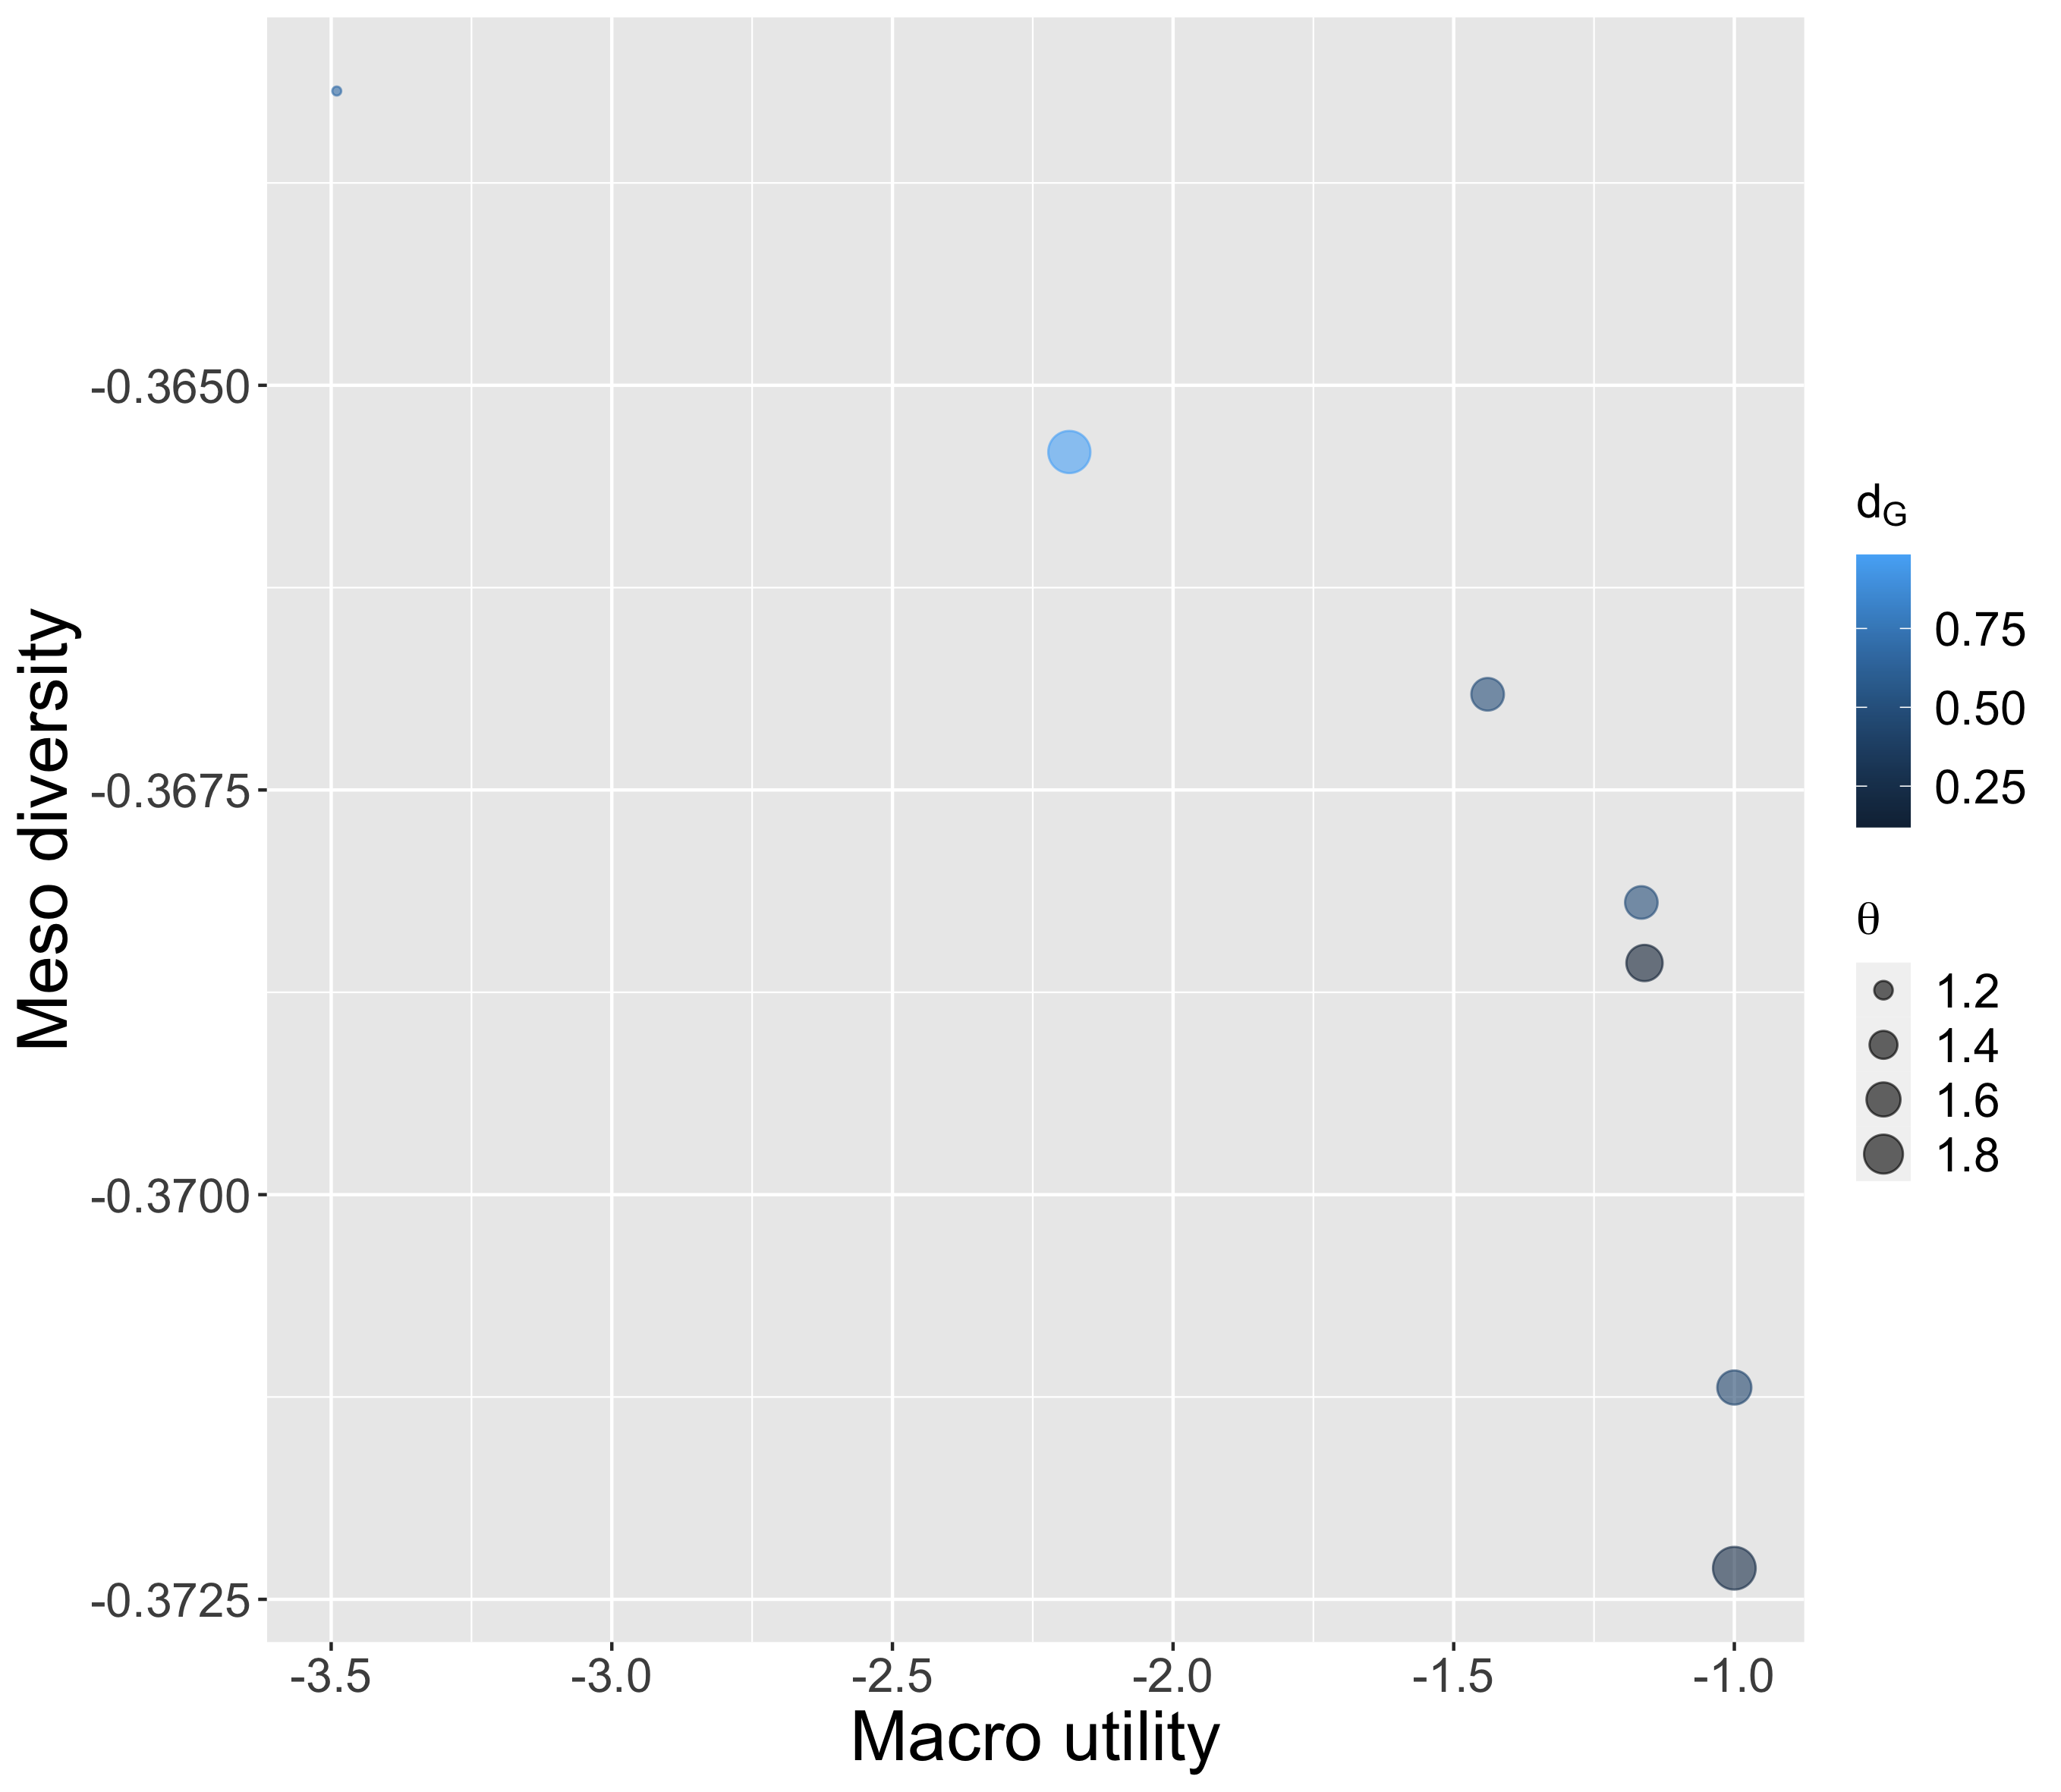
\includegraphics[width=0.7\linewidth]{../figures/paretoDiversity-Fitness_colordG_sizetheta}
\end{center}

 \footnotesize

\textit{\textbf{Bi-objective optimisation} of indicators at both scales: aggregated utility at the macro scale and diversity of innovations within urban areas}

}


\sframe{Diversity search}{


\begin{center}
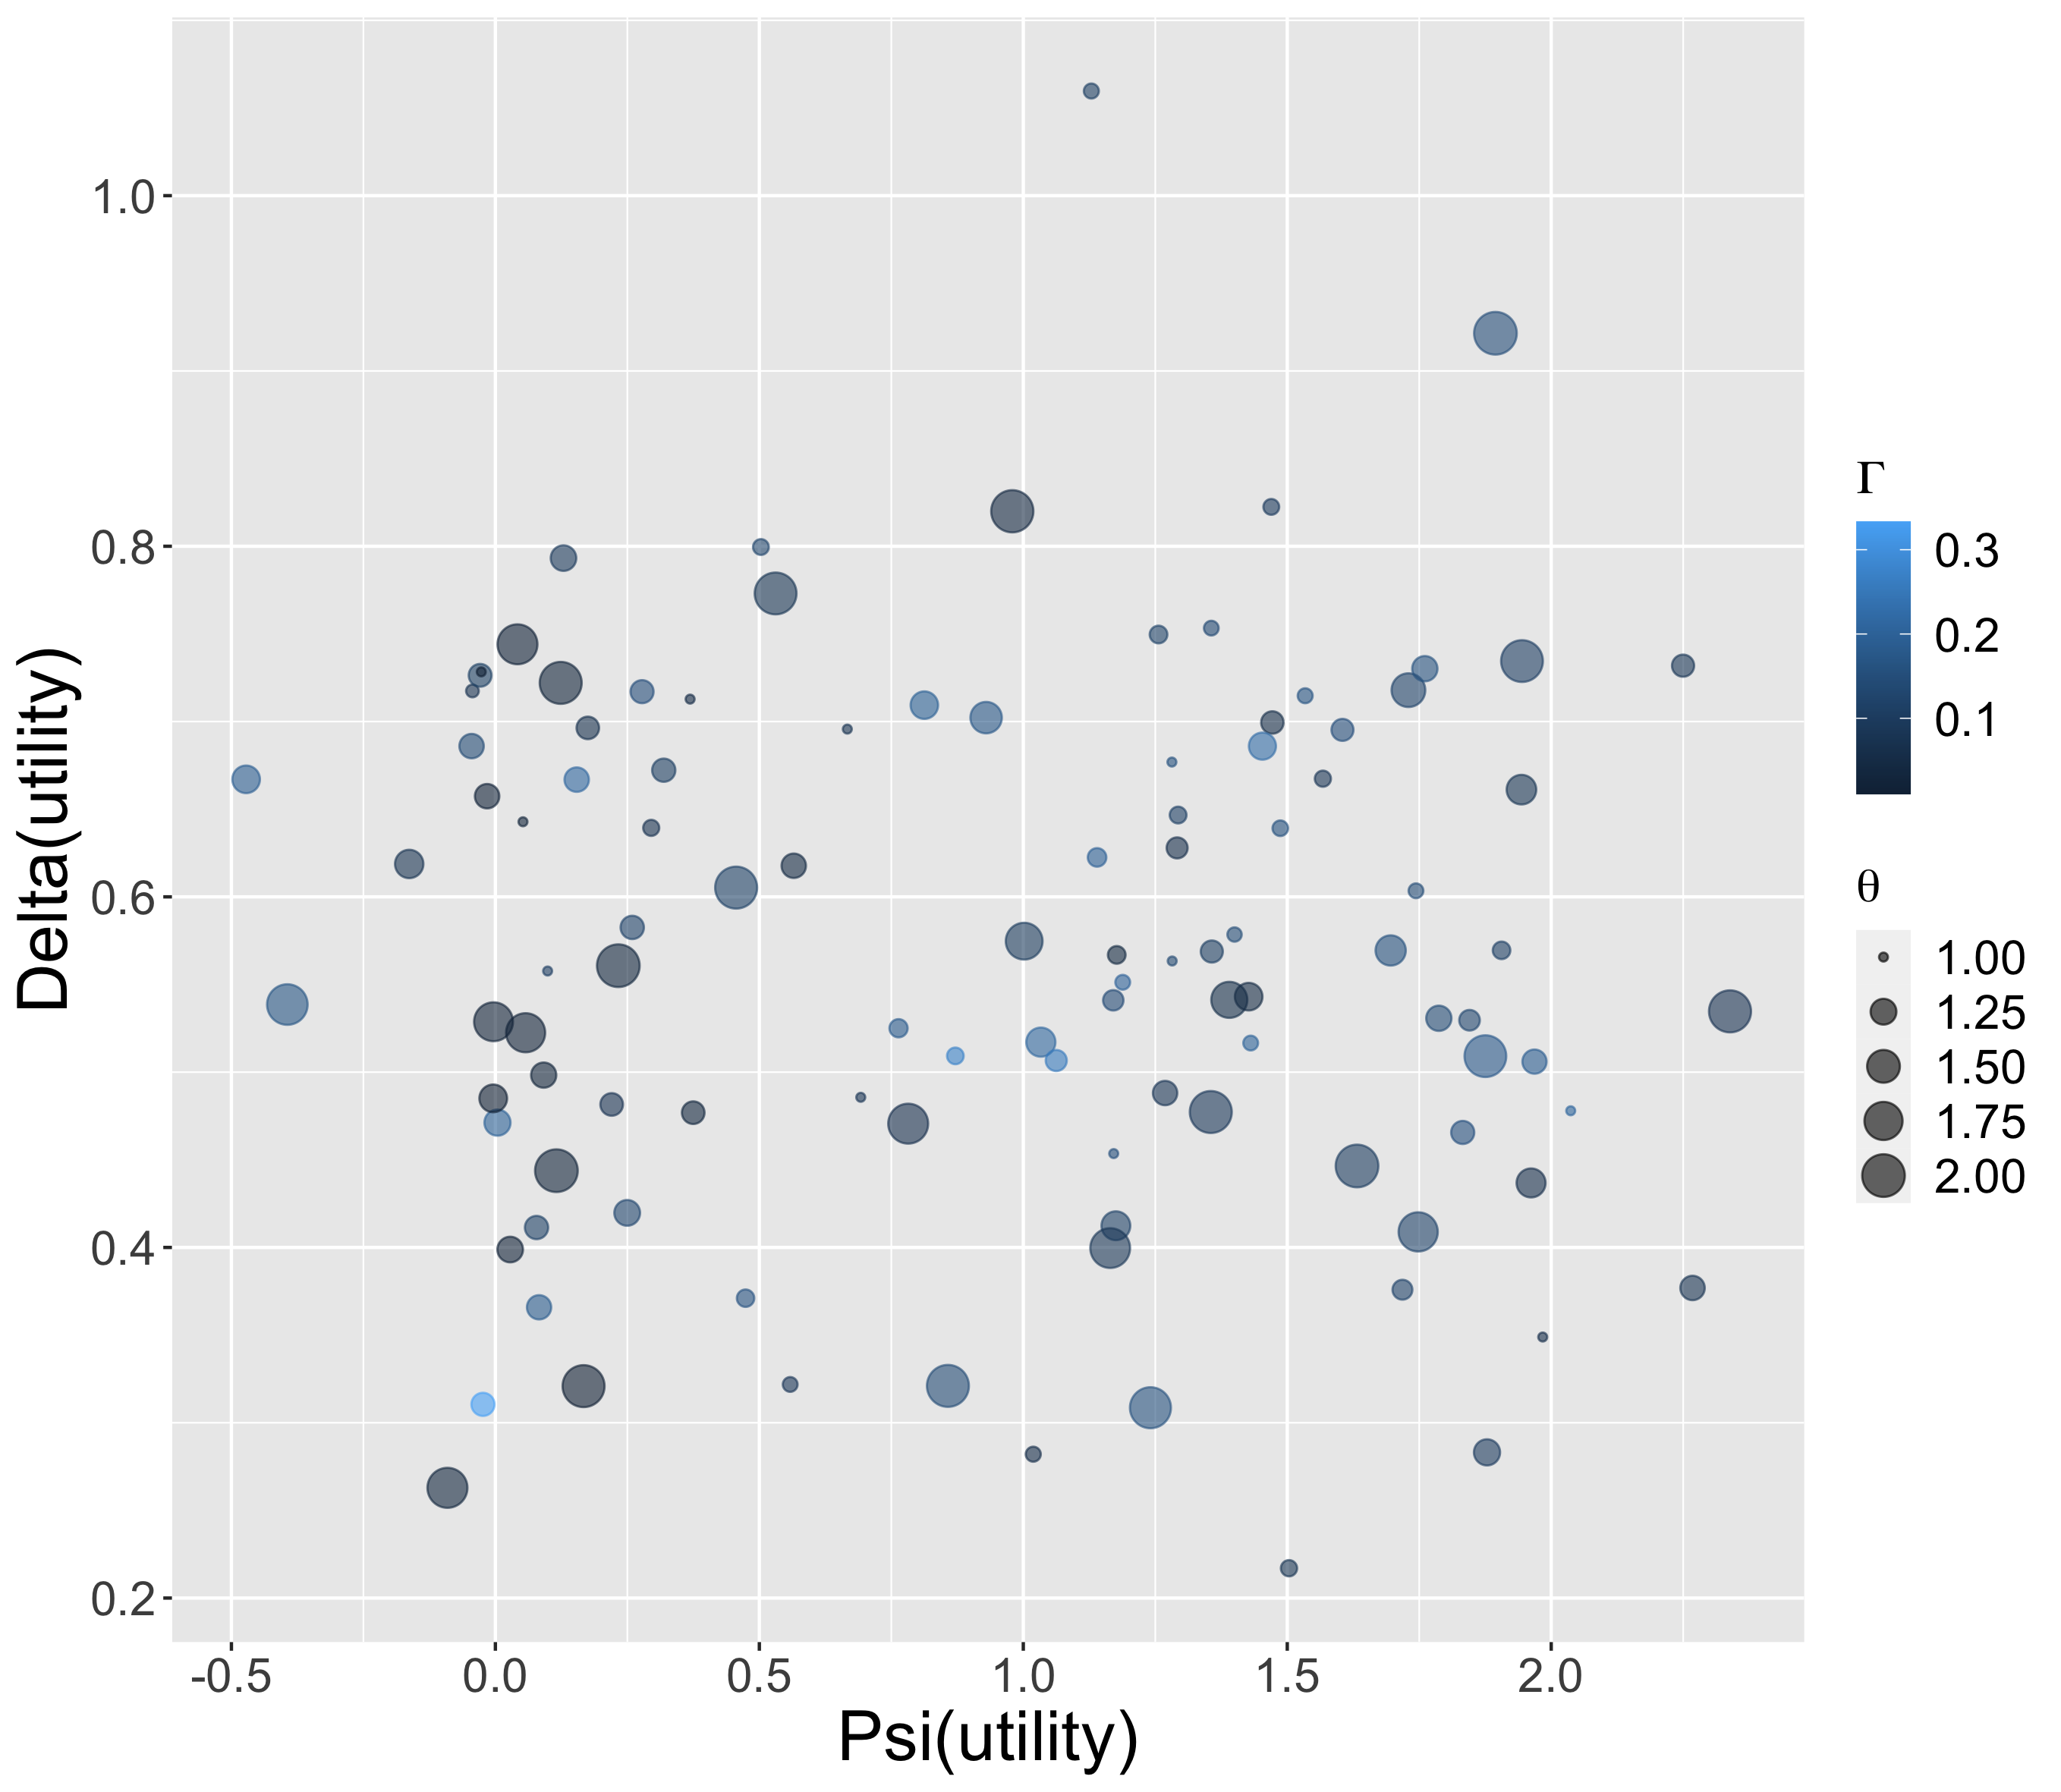
\includegraphics[width=0.64\linewidth]{../figures/pse-psi-delta-utility_colorGamma_sizetheta.png}
\end{center}

 \footnotesize

\textit{Application of the \textbf{PSE diversity search algorithm} \cite{cherel2015beyond} to obtain the feasible space of emergence regimes: downward causation always occurs ($\Delta > 0$), many regimes with causal emergence ($\Psi > 0$) and with autonomy between scales ($\Gamma \sim 0$).}

}


\sframe{Discussion}{

\justify

$\rightarrow$ \textbf{Main results:} proof-of-concept for a \textbf{bi-objective optimisation across scales}, towards policy applications; \textbf{diversity of emergence regimes} produced by the model.
			
\bigskip
				
$\rightarrow$ Possible extensions: higher dimension of the innovation space, economic structure for companies, coupling with economic agent-based models, migration of ideas (employees) between urban areas, bottom-up feedback through a change of macro parameters.

\bigskip
				
$\rightarrow$ Future application on real urban systems requires innovation data across scales: adaptation of the model to fit specific data, patent data only a proxy of innovation, firm data not open.

\bigskip

\textbf{Conclusion: } a first step towards \textbf{multi-scalar integrated models} for sustainable urban and territorial policies.

}









%%%%%%%%%%%%%%%%%%%%%
\begin{frame}[allowframebreaks]
\frametitle{References}
\bibliographystyle{apalike}
\bibliography{../biblio}
\end{frame}
%%%%%%%%%%%%%%%%%%%%%%%%%%%%




\end{document}









